\chapter{Overview of a DBMS}

This chapter will give a general overview of the structure of a centralized \textbf{DBMS} (\textbf{Data Base Management System}) based on the relational data model, describing its components and their respective functionalities.

\section{Architecture}

A database is a collection of homogeneous sets of data, with relationships defined among them, stored in permanent memory, and used via a DBMS.

\BoxDef{DBMS}{
A DBMS is a software that provides the following functionalities:
\begin{itemize}
    \item A language to describe the \textbf{schema} of the database (a collection of definitions that describe the data structures), restrictions on the allowed data types, and the relationships among data sets;
    \item The data structures for storage and efficient retrieval of large amounts of data;
    \item A language to guarantee secure access to the data only to authorized users;
    \item A \textbf{transactions} mechanism to protect data from HW/SW malfunctions and errors during concurrent access.
\end{itemize}
}

The architecture of a DBMS provides the following basic components:
\begin{itemize}
    \item The \textbf{Storage Engine}, which includes modules supporting:
    \begin{itemize}
        \item \textbf{Permanent Memory Manager};
        \item \textbf{Buffer Manager};
        \item \textbf{Storage Structures Manager};
        \item \textbf{Access Methods Manager};
        \item \textbf{Transaction and Recovery Manager};
        \item \textbf{Concurrency Manager}.
    \end{itemize}

    \item The \textbf{Relational Engine}, which includes modules supporting:
    \begin{itemize}
        \item \textbf{Data Definition Language};
        \item \textbf{Query Manager};
        \item \textbf{Catalog Manager}.
    \end{itemize}
\end{itemize}
In real systems the functionalities of these modules are not completely separated in different components (as in Figure \ref{fig:DBMS_schema}), but this overview can help in understanding the purpose of each of them. 

\begin{figure}[h]
    \centering
    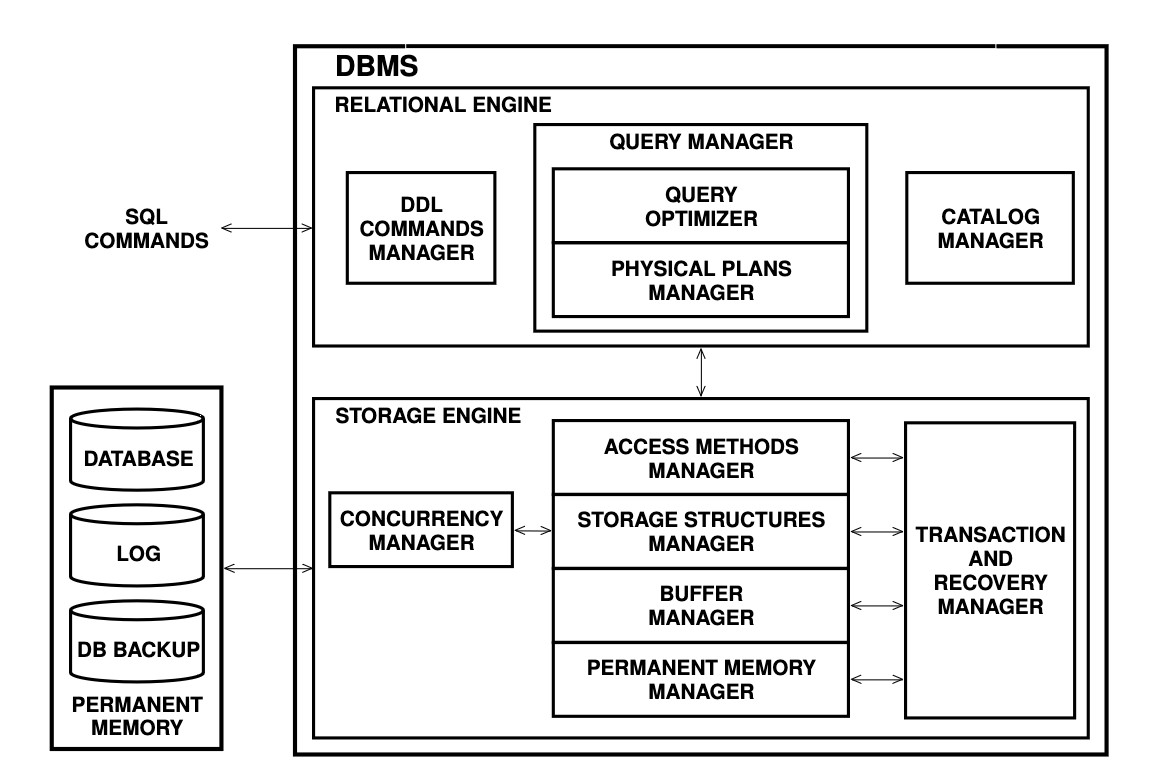
\includegraphics[width=0.75\linewidth]{img/DBMS schema.png}
    \caption{The architecture of a DBMS.}
    \label{fig:DBMS_schema}
\end{figure}

\subsection{Permanent Memory Manager}

The PMM manages page allocation and deallocation on disk storage. It hides the disk characteristics and the operating system, as it provides an abstraction of the memory as a a set of databases, each consisting of a set of logical files of \textbf{physical pages} (or blocks) of fixed size. The physical pages of a file are numbered consecutively starting from 0, and their number can grow dynamically with the only limitation being the available space in the permanent memory.